\documentclass[a4paper,oneside,12pt]{article}
\usepackage[french]{babel}
\usepackage[utf8]{inputenc}
\usepackage[french]{babel}
%\usepackage{fullpage}
%\usepackage{xkeyval}
\usepackage{rotating}
\usepackage{amsmath}
\usepackage{amsfonts,amssymb}
\usepackage{float}
\usepackage{fancyhdr}
\usepackage{graphicx}
\usepackage{verbatim}
\usepackage{lastpage}
\usepackage{pstricks}
%\usepackage{aeguill}
\usepackage{color}
\usepackage{multicol}
\usepackage{mathenv}
\usepackage{amssymb}
\setlength{\headsep}{1cm}

%%%%%%%%%%%%%%%% Variables %%%%%%%%%%%%%%%%
\def\titre{Exploitation simultanée des processeurs et de l'accélérateur GPU}
\def\titregauche{Projet CPU\&GPU}
\def\titredroite{Rapport de projet}
\def\filiere{informatique}
\def\annee{$2^{eme}$}  % $1^{ere}$, $2^{eme}$ ou $3^{eme}$
\def\anneescolaire{2012}
\def\equipe{Jiang Lun \\ Rouxel Quentin}

%%%%%%%%%%%%%%%%%%%%%%%%%%%%%%%%%%%%%%%%%%%
\pagestyle{fancy} \lhead{\textsc{\titregauche}} 
\rfoot{\textit{Ann\'ee \anneescolaire}}\rhead{\textsc{\titredroite}}\cfoot{\thepage/\pageref{LastPage}}
\renewcommand{\headrulewidth}{0.4pt}
\renewcommand{\footrulewidth}{0.4pt}

\newcommand{\HRule}{\rule{\linewidth}{0.5mm}}

\begin{document}

\begin{titlepage}

\begin{center}

\begin{center}
\rotatebox{0}{\scalebox{1}[1]{
\includegraphics[width=5cm]{Logo_ENSEIRB-MATMECA.png}}}
\end{center}
~\\
~\\
~\\
\textsc{\LARGE ENSEIRB-MATMECA}\\[1cm]

\textsc{\Large {Fili\`ere \filiere, \annee ann\'ee}}\\[0.5cm]

% Title
\HRule \\[0.4cm]
{ \huge \bfseries \titre}\\[0.4cm]


\HRule \\[1.5cm]

% Author and supervisor
\begin{minipage}{0.4\textwidth}
\begin{flushleft} \large
\vspace{-1.0cm}
\emph{Auteurs:}\\
\equipe
\vspace{0.5cm}
\end{flushleft}
\end{minipage}
\begin{minipage}{0.4\textwidth}
\begin{flushright} \large
%\emph{Encadrant:} \\
%\encadrant
\end{flushright}
\end{minipage}

\vfill

% Bottom of the page
{\large \today}

\end{center}

\end{titlepage}

\section*{Problèmes rencontrés}

La difficulté majeur de ce projet est vraisemblablement la manipulation des indices.
Ces derniers doivent pour des raisons de performances au niveau du GPU être alignés le plus souvent sur
un multiple de 16 octets.
Dans un premier temps, nous avons utilisé soit uniquement le processeur, 
soit uniquement la carte graphique afin de tester si nos indices étaient correctes. Le nombre d'erreurs
engendrées a également été pour nous un bon outil de debogage lors de l'utilisation des deux unités de calcul.
Cependant, les indices trouvés ne marchaient pas lors de l'utilisation simultanée des deux unités.
Le nombre d'erreurs étant égale au nombre d'éléments d'une ligne, nous avons rapidement conclu
que notre problème venait du recouvrement des bords à la séparation CPU GPU. Lors du rapatriement des données
calculées sur le GPU, la ligne du bord supérieur écrasais la dernière ligne calculée par le CPU.\\
Une fois ce problème corrigé, le calcul d'une itération sur les deux unités de calcul fonctionnait parfaitement.\\\\

Le passage à plusieurs itérations a simplement nécessité l'allocation d'une troisième matrice contenant les valeurs initiales
afin de calculer à la fin le résultat avec le programme séquentiel puisque les deux matrices $input$ et $output$ 
sont modifiées au cours du calcul.\\
La propagation des bords entre le CPU et le GPU s'est déroulée sans encombre.\\\\

A ce stade, le programme n'utilisant qu'un seul CPU simultanément et le GPU, les accélérations (speedup) obtenus étaient
relativement stables. Mais après la parallélisation de la partie CPU à l'aide de OpenMP, 
les accélérations n'était alors plus du tout stable. Il nous a fallu fixer le nombre de threads générés 
par OpenMP à 14 pour retrouver des performances assez stable. Ce problème était certainement dû à 
une concurrence entre le thread principal contrôlant la communication avec la carte graphique et les 
autres thread de calculs sur un même cœur.

\section*{Résultats}

Au cours de l'implémentation, nous avons pu constater des performances croissantes 
sur notre matrice de test (4096*4096, 50 itérations) :\\\\
\begin{itemize}
\item Version GPU seul : accélération $\approx$ 3.87 (2.46 Go/s) 
\item Version CPU parallélisé : accélération $\approx$ 3.93 (2.50 Go/s)
\item Version GPU + CPU non parallélisé (meilleur partage trouvé) : accélération $\approx$ 4.63 (2.97 Go/s)
\item Version GPU + CPU parallélisé (meilleur partage trouvé) : accélération $\approx$ 6.50 (4.14 Go/s)\\\\
\end{itemize}

Nous avons également écrit un script de test en PHP afin de générer un graphique rendant compte de l'évolution de l'accélération 
en fonction du nombre d'itération et de la répartition CPU/GPU. Ci dessous un aperçu du graphique 3d généré 
à l'aide de GNUplot.
~~\\\\
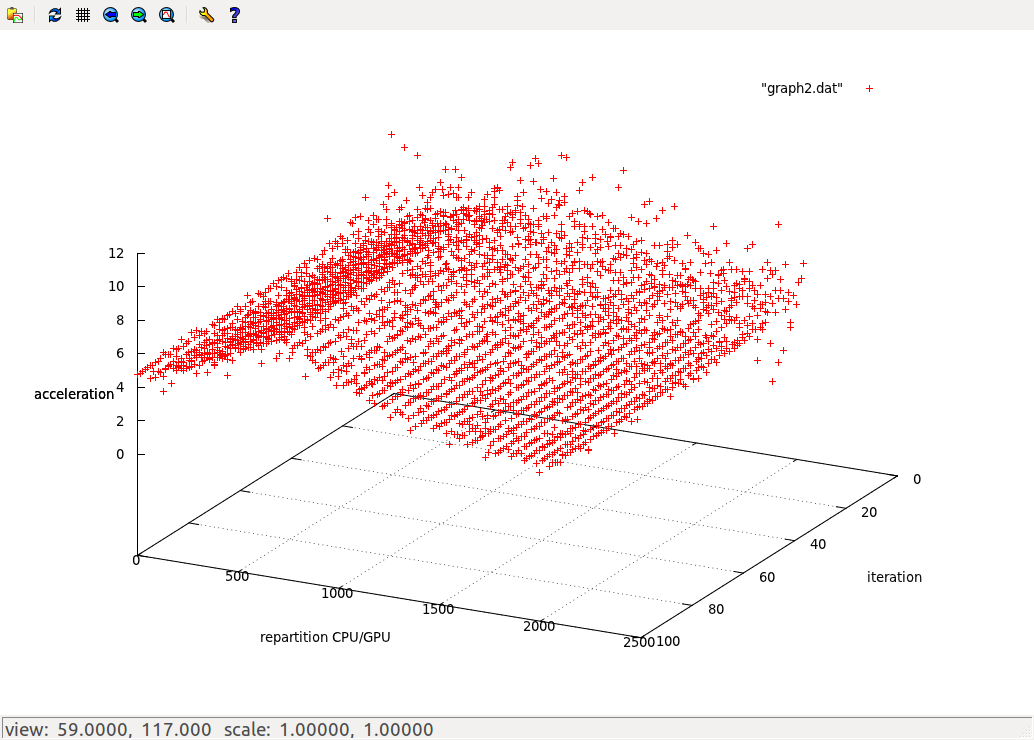
\includegraphics[width=1\textwidth]{graph1.png}\\
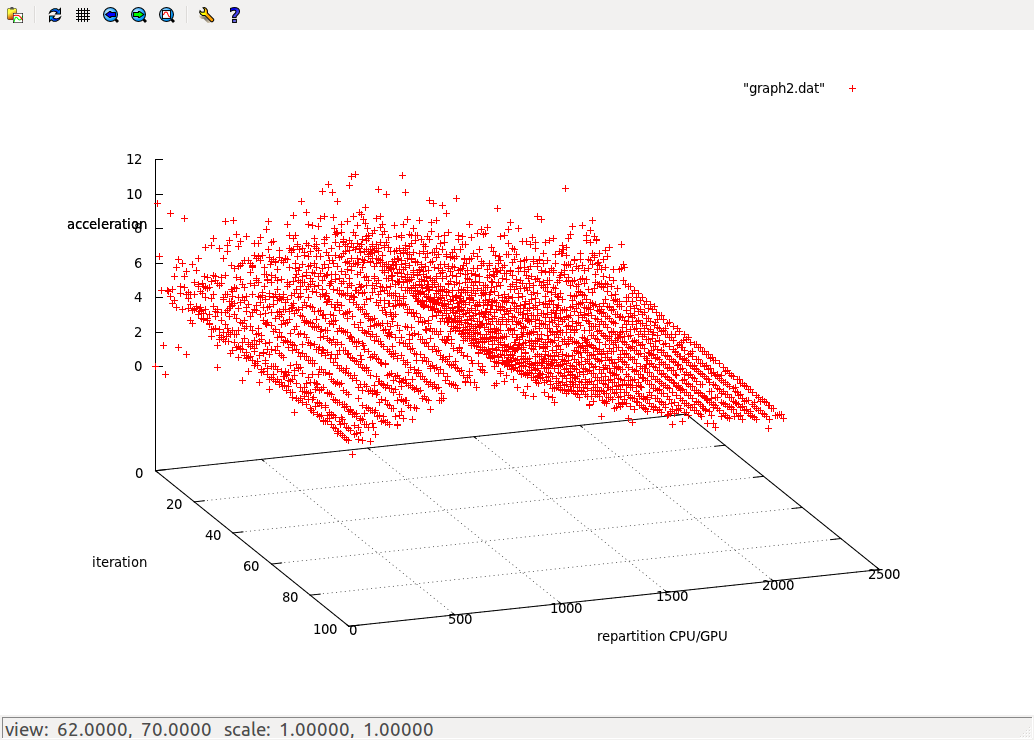
\includegraphics[width=1\textwidth]{graph2.png}\\

Le graphique est disponible à partir du fichier \textit{graph.dat} situé à la racine du projet.

\section*{Conclusion}

Au final les accélérations sont plutôt satisfaisantes. Néanmoins, nous pensons que de meilleurs performances sont
possible en tentant de minimiser l'impacte du transfert des bords à chaque itération. La solution serait de considérer
un bord plus large et de ne le transférer que plus rarement pour rentabiliser le coût du transfert.

\end{document}

